\subsection{Optimisation algorithms for task allocation and resource allocation}
\label{section:algorithm_summaries}
%%%%%%%%%%%%%%%%
\newcommand{\varAction}[2]{\varSymbol{a}{#1}{#2}}
\newcommand{\functionExec}[2]{
	\ifx &#1&
	\texttt{exec}(\varAtomicTask{}{})
	\else
	\texttt{exec}(#1, #2)
	\fi
}
\newcommand{\functionAlloc}[2]{
	\ifx &#1&
	\texttt{alloc}(\varAtomicTask{}{}, \varAgent{}{})
	\else
	\texttt{alloc}(#1, #2)
	\fi
}
\newcommand{\functionInfo}[2]{
	\ifx &#1&
	\texttt{info}(\varAgent{}{})
	\else
	\texttt{info}(#1)
	\fi
}
\newcommand{\functionLink}[2]{
	\ifx &#1&
	\texttt{link}(\varAgent{}{})
	\else
	\texttt{link}(#1)
	\fi
}
\newcommand{\functionATARIA}[2]{
	\functionSignature{
		\texttt{ataria}
	}{
		\varAgent{}{}, \varAtomicTask{}{}
	}
}	
\newcommand{\varTaskValue}[2]{taskval}
\newcommand{\functionATARIAAction}[2]{
\ifx &#1&
	\functionSignature{\texttt{ataria-action}}{\varAgent{}{}, \varAtomicTask{}{}}
\else
	\functionSignature{\texttt{ataria-action}}{\varAgent{#1}{}, \varAtomicTask{#2}{}}
\fi
}	
\newcommand{\functionATARIAUpdate}[2]{
\ifx &#1&
\functionSignature{\texttt{ataria-update}}{\varAgent{}{}, \varTaskValue{}{\varAtomicTask{}{}, \varTaskValue{}{}}}
\else
\functionSignature{\texttt{ataria-update}}{\varAgent{#1}{}, \varAtomicTask{#2}{}, \varTaskValue{}{}}
\fi
}	
\newcommand{\formalATARIA}[2]{
	\functionFormal{\texttt{ataria}_{\varAgent{}{}}}
	{\setAtomicTask{}{} \times \setAgents{}{}}
	{
		\texttt{exec}(\setAtomicTask{}{})
		\times \texttt{alloc}(\setAtomicTask{}{}, \setAgents{}{})
		\times \texttt{info}(\setAgents{}{})
		\times \texttt{link}(\setAgents{}{})
	}
}
\newcommand{\functionMGRAOWeighting}[2]{\texttt{mgrao-weight}(\varAtomicTask{}{}, \varAgent{self}{})}
\newcommand{\formalMGRAOWeighting}[2]{
	\functionFormal{\texttt{mgrao-weight}_{\varAgent{}{}}}
	{\setAtomicTask{}{} \times \setRealNumbers{}{}}
	{
		\setRealNumbers{}{}
	}
}
\newcommand{\functionMGRAOUpdate}[2]{
\ifx &#1&
	\functionSignature{\texttt{mgrao-update}}{\varAgent{}{}, \varAtomicTask{}{}, \functionTaskAbsoluteValue{}{}}
\else
\functionSignature{\texttt{mgrao-update}}{\varAgent{}{}, \varAtomicTask{}{}, \functionTaskAbsoluteValue{}{}}
\fi
}
\newcommand{\formalMGRAOUpdate}[2]{
	\functionFormal{\texttt{mgrao-update}_{\varAgent{}{}}}
	{\setAtomicTask{}{} \times \setRealNumbers{}{}}
	{
		\setRealNumbers{}{}
	}
}
%%%%%%%%%%%%

The \acronymATARIA{}{} algorithm enables agents in the system to learn the best actions to take given their current state. This ranges from deciding which other agents to allocate tasks to and obtain the best composite task values, to exploring the system for other agents, while adapting connectivity to handle network disruption. An agent uses the \acronymATARIA{}{} algorithm to choose an action to take, which can be one of the following,
\begin{enumerate}
	\item $\functionExec{}{}$, The agent will execute the atomic task $\varAtomicTask{}{}$ itself.
	\item $\functionAlloc{}{}$, the agent will allocate the atomic task $\varAtomicTask{}{}$ to another agent $\varAgent{}{}$.
	\item $\functionInfo{}{}$, the agent will request information from another agent $\varAgent{}{}$.
	\item $\functionLink{}{}$, the agent will allocate resources to hold information on the agent $\varAgent{}{}$ and maintain a connection.
\end{enumerate}
\begin{figure}[ht]
	\centering
	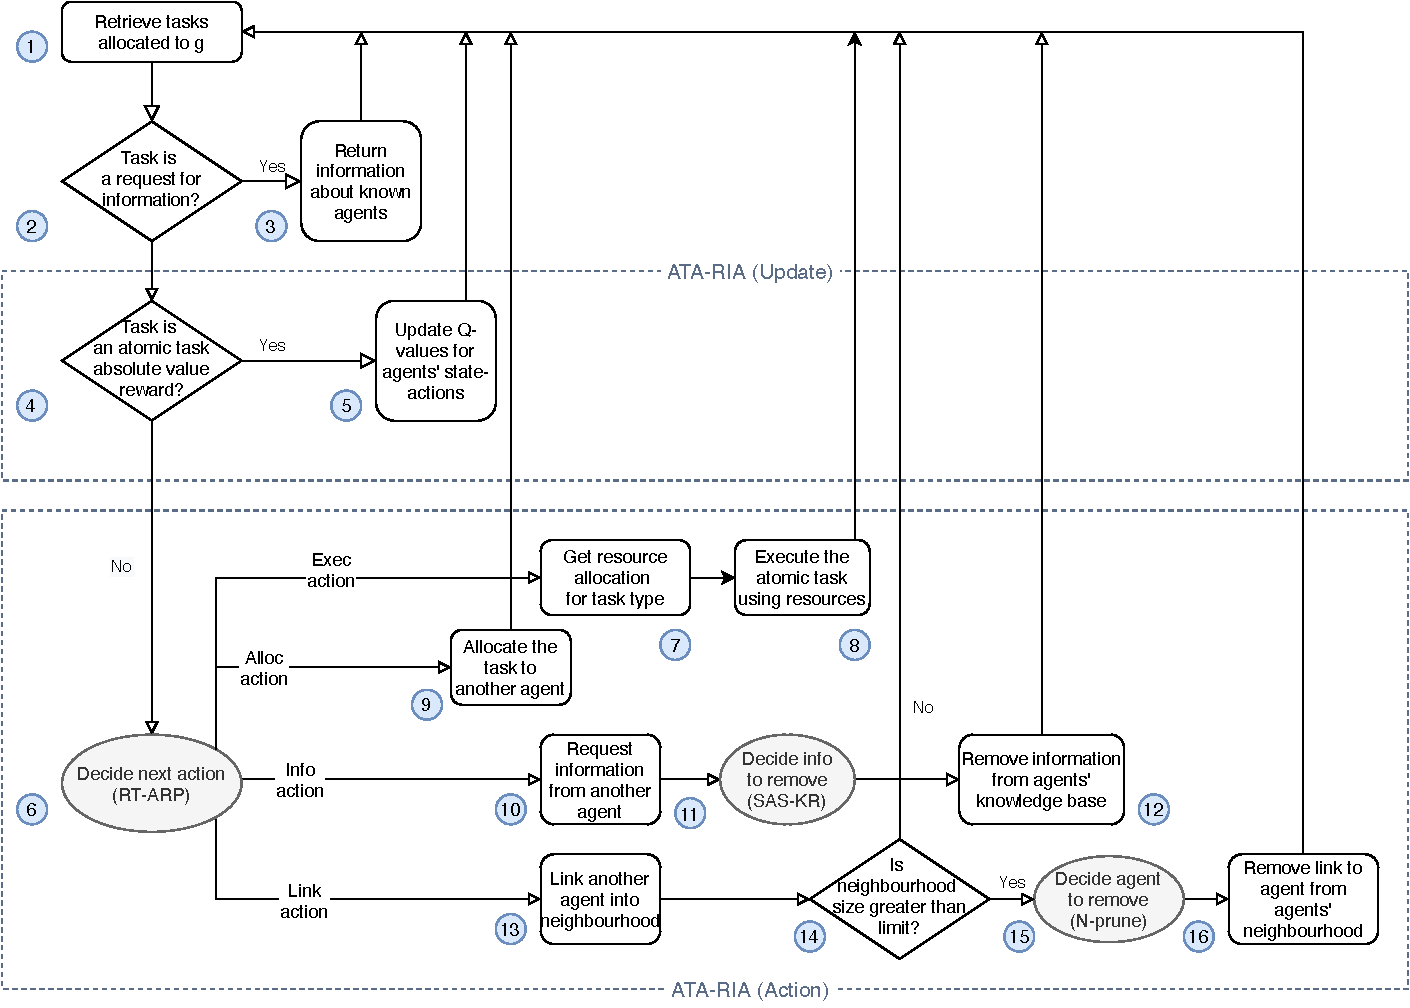
\includegraphics[width=0.8\linewidth, trim={65pt 0pt 65pt 0pt, clip}]{ataria-simplified}
	\caption{\textbf{Simplified \acronymATARIA{}{} flowchart}. The diagram shows the decision-making and actions taken by an agent using the \acronymATARIA{}{}  algorithm. \newline
		\textbf{(1)} The agent starts with the current tasks is has to process. \newline
		\textbf{(2-3)} If the task is a request for information, the agent returns details of an agent from its knowledge base to the requester. \newline
		\textbf{(4-5)} If the task is a reward sent to the agent for completing a previous atomic task, the Q-values for the agents state-actions are updated. \newline
		\textbf{(6)} Otherwise, an action is chosen using the RT-ARP sub-algorithm. This algorithm selects the optimal action given the agents current state, based on a set of Q-learning values derived from past actions, and historical rewards.  \newline
		\textbf{(7)} If the selected action is an \texttt{exec} action, the agent simply executes the task itself. \newline
		\textbf{(8)} If the action is an \texttt{alloc} action, the task is allocated to another agent to complete, chosen from the agents' neighbourhood. \newline
		\textbf{(9-11)} For an \texttt{info} action, the agent will send a request to another agent in its neighbourhood to return information on additional agents in the system. If the information it gets back increases its knowledge base beyond the size limit, it will judge which is the least important information using the SAS-KR algorithm, and remove that from its knowledge base. \newline
		\textbf{(12-15)} For a \texttt{link} action, the agent will link the selected agent from its knowledge base into its neighbourhood. It will perform any pruning required to maintain the neighbourhood within its resource limitations by choosing to remove the agent that has provided the least task quality in the past. \newline
}
	\label{fig:ataria-simplified}
\end{figure}

The \acronymATARIA{}{} algorithm learns to select the actions that generate the best composite task values, and adapt the choice of action depending on how good the composite task values are in comparison to the historical values through the updating of Q-values in its temporal-update algorithm. The algorithm will select one of the possible actions for the agent $\varAgent{}{}$, given it has non-completed, allocated tasks $\setAtomicTask{}{}$, and knows of other agents $\setAgents{}{}$ through the function,
\begin{equation}
	\label{eq:ataria}\formalATARIA{}{}
\end{equation}

To enable agents to form task-paths we allow atomic tasks that have been allocated to an agent to be either executed by that agent, or re-allocated to further agents, through running the \acronymATARIA{}{} algorithm. Figure \ref{fig:arc-flow} illustrates a task-path where there are two re-allocations made before a specific atomic task is allocated to an agent that completes the task by taking a measurement.
\begin{figure}[ht]
	\centering
	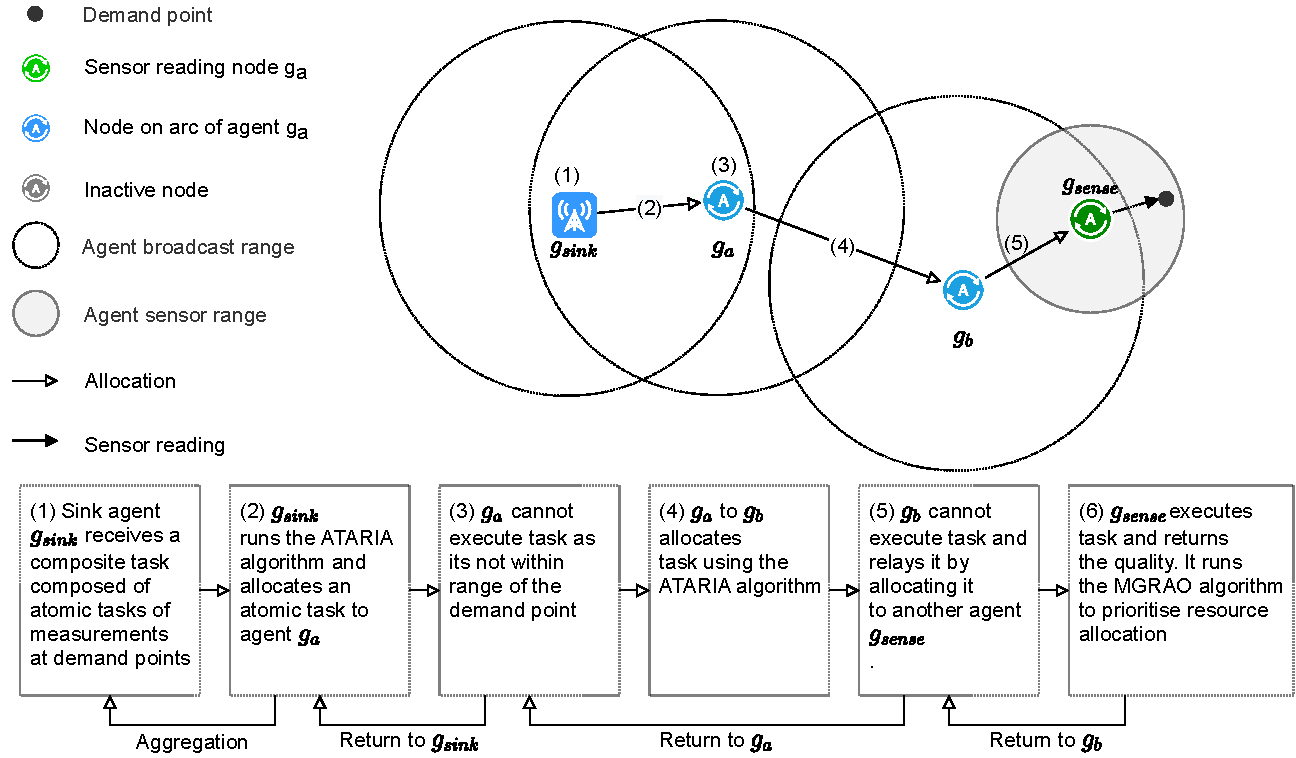
\includegraphics[width=0.8\linewidth, trim={25pt 0pt 25pt 0pt, clip}]{arc-flow}
	\caption{\textbf{Allocation along a task-path}. This diagram illustrates how allocations can be relayed along a task-path using successive applications of the \acronymATARIA{}{} algorithm.}
	\label{fig:arc-flow}
\end{figure}